\documentclass[a4paper, 11pt]{report}
\usepackage{../preamble}


\begin{document}

\doctype{Homework}
\coursetitle{Convex Optimization and applications in Machine Learning}
\semester{MVA Fall 2019}
\instructor{Alexandre d'Aspremont}
\student{Antoine Moulin}
\worknumber{1}
\workdate{October 14}

\maketitle

The following exercises can be found in the book: \textbf{Convex Optimization} by Lieven Vandenberghe and Stephen Boyd.

\section*{Exercise 2.12}

Which of the following sets are convex?

\begin{itemize}
	\item[(a)] A \emph{slab}, \ie, a set of the form $\set{x \in \Rn}{\alpha \leq a^{T}x \leq \beta}$.
	
	\item[(b)] A \emph{rectangle}, \ie, a set of the form $\set{x \in \Rn}{\forall i \in [\![ 1, n ]\!], \alpha_{i} \leq x_{i} \leq \beta_{i}}$. A rectangle is sometimes called a \emph{hyperrectangle} when $n > 2$.
	
	\item[(c)] A \emph{wedge}, \ie, $\set{x \in \Rn}{a_{1}^{T}x \leq b_{1}, a_{2}^{T}x \leq b_{2}}$.
	
	\item[(d)] The set of points closer to a given point than a given set, \ie,
	\[ \set{x \in \Rn}{\forall y \in S, \norm{x - x_{0}}{2} \leq \norm{x - y}{2}} \]
	\noindent where $S \subseteq \Rn$.
	
	\item[(e)] The set of points closer to one set than another, \ie,
	\[ \set{x \in \Rn}{\dist(x, S) \leq \dist(x, T)} \]
	\noindent where $S, T \subseteq \Rn$, and
	\[ \dist(x, S) = \inf \set{\norm{x - z}{2}}{z \in S} \]
	
	\item[(f)] [HUL93, volume 1, page 93] The set $\set{x \in \Rn}{x + S_{2} \subseteq S_{1}}$, where $S_{1}, S_{2} \subseteq \Rn$ with $S_{1}$ convex.
	
	\item[(g)] The set of points whose distance to $a$ does not exceed a fixed fraction $\theta$ of the distance to $b$, \ie, the set $\set{x \in \Rn}{\norm{x - a}{2} \leq \theta \norm{x - b}{2}}$. You can assume $a \neq b$ and $0 \leq \theta \leq 1$.
\end{itemize}

\noindent \textbf{Solution.}

\begin{itemize}
    \item[(a)] According to the definition, a slab is an intersection of two halfspaces (convex sets). An intersection of convex sets is convex, hence a slab is convex.
    
    \item[(b)] A rectangle in dimension $n$ is the intersection of $n$ slabs. For $i \in [\![ 1, n  ]\!]$, let denote by $e_{i}$ the vector whose $i$-th component is $1$ and the others are $0$. We have:
    \[ \set{x \in \Rn}{\forall i \in [\![ 1, n ]\!], \alpha_{i} \leq x_{i} \leq \beta_{i}} = \bigcap_{i=1}^{n} \set{x \in \Rn}{\alpha_{i} \leq e_{i}^{T}x \leq \beta_{i}} \]
    
    A slab is convex (see (a)) and an intersection of convex sets is convex. Thus, a rectangle is convex.
    
    \item[(c)] As in (a), a wedge is the intersection of two halfspaces, thus it is convex.
    
    \item[(d)] Let $y \in S$. Let show that $C(y) = \set{x \in \Rn}{\norm{x - x_{0}}{2} \leq \norm{x - y}{2}}$ is a halfspace, hence a convex set. With $n = 2$, we clearly see that the split is made by the perpendicular bisector of the segment $[x_{0}, y]$. Let $x \in C(y)$.
    
    \begin{equation*}
        \begin{split}
            \norm{x - x_{0}}{2} \leq \norm{x - y}{2} &\text{ iff } \norm{x - x_{0}}{2}^{2} \leq \norm{x - y}{2}^{2} \\
            &\text{ iff } \left( x - x_{0} \right)^{T} \left( x - x_{0} \right) \leq \left( x - y \right)^{T} \left( x - y \right) \\
            &\text{ iff } - 2 x_{0}^{T}x + \norm{x_{0}}{2}^{2} \leq - 2 y^{T}x + \norm{y}{2}^{2} \\
            &\text{ iff } \left( y - x_{0} \right)^{T}x \leq \frac{\norm{y}{2}^{2} - \norm{x_{0}}{2}^{2}}{2}
        \end{split}
    \end{equation*}


Defining $a = y - x_{0}$ and $b = \frac{\norm{y}{2}^{2} - \norm{x_{0}}{2}^{2}}{2}$, we see that $C(y)$ is a halfspace, hence convex.

We have $\set{x \in \Rn}{\forall y \in S, \norm{x - x_{0}}{2} \leq \norm{x - y}{2}} = \displaystyle\bigcap_{y \in S} C(y)$. An intersection of convex sets is convex, hence the initial set is convex.

    \item[(e)] In general, the set $A = \set{x \in \Rn}{\dist(x, S) \leq \dist(x, T)}$ is not convex. Here is an example in which it is not convex:
    
    \begin{figure*}[!h]
    \centering
    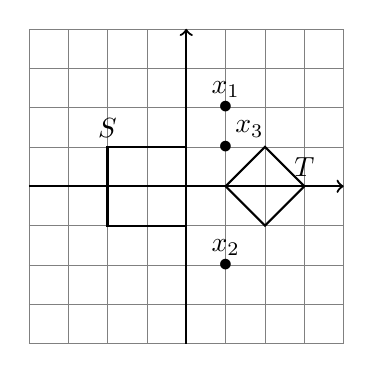
\begin{tikzpicture}
    \draw[step=0.5cm, very thin, gray] (-2, -2) grid (2, 2);
    \draw[thick, ->] (-2, 0) -- (2, 0);
    \draw[thick, ->] (0, -2) -- (0, 2);
    
    \draw[thick] (-1, -0.5) rectangle (0, 0.5); 
    \draw (-1, 0.5) node[above]{$S$};
    
    \draw[thick] (0.5, 0) -- (1, 0.5) -- (1.5, 0) -- (1, -0.5) -- cycle;
    \draw (1.5, 0) node[above]{$T$};

    \draw (0.5, 1) node{$\bullet$} node[above]{$x_{1}$};
    \draw (0.5, -1) node{$\bullet$} node[above]{$x_{2}$};
    \draw (0.5, 0.5) node{$\bullet$} node[above right]{$x_{3}$};
    \end{tikzpicture}
    \caption{Example in which the set $A$ is not convex.}
    \end{figure*}
    
    Here, $x_{1}$ and $x_{2}$ are in the set $A$ (because for $i \in \left\{ 1, 2 \right\}$, $\dist(x_{i}, S) = \dist(x_{i}, T)$), but $x_{3}$ - which is in the segment $[x_{1}, x_{2}]$ - is not. Hence, the set $A$ is not convex.
    
    \item[(f)] Let $C = \set{x \in \Rn}{ x + S_{2} \subseteq S_{1}}$, $u, v \in C, \theta \in [0, 1]$  and let show that $\left( \theta u + (1 - \theta) v \right) + S_{2} \subseteq S_{1}$. Let $s \in S_{2}$. We have:
    
    \[ \theta u + (1 - \theta) v + s = \theta(\underbrace{u + s}_{\in S_{1}}) + (1 - \theta)(\underbrace{v + s}_{\in S_{1}}) \in S_{1} \]
    
    $u + s \in S_{1}$ because $u \in C$, $v + s \in S_{1}$ because $v \in C$ and the convex combination is in $S_{1}$ as well because $S_{1}$ is convex. Hence, $C$ is convex.
    
    \item[(g)] Let $C = \set{x \in \Rn}{\norm{x - a}{2} \leq \theta \norm{x - b}{2}}$. Let $x \in \Rn$.
    
    \begin{equation*}
        \begin{split}
            x \in C &\text{ iff } \norm{x - a}{2} \leq \theta \norm{x - b}{2} \\
            &\text{ iff } \left( x - a \right)^{T} \left( x - a \right) \leq \theta^{2} \left( x - b \right)^{T} \left( x - b \right) \\
            &\text{ iff } \norm{x}{2}^{2} - 2a^{T}x + \norm{a}{2}^{2} \leq \theta^{2} \norm{x}{2}^{2} - 2 \theta^{2}b^{T}x + \theta^{2}\norm{b}{2}^{2} \\
            &\text{ iff } f(x) \triangleq (1 - \theta^{2}) \norm{x}{2}^{2} + 2(\theta^{2}b - a)^{T}x \leq \theta^{2} \norm{b}{2}^{2} - \norm{a}{2}^{2}
        \end{split}
    \end{equation*}
    
    The function $f$ is convex and $C$ is a sublevel set of $f$. Hence, $C$ is convex.
\end{itemize}



\section*{Exercise 3.21}

\textit{Pointwise maximum and supremum}. Show that the following functions $f: \Rn \longrightarrow \Rn$ are convex.

\begin{itemize}
    \item[(a)] $f(x) = \max_{i \in [\![ 1, k ]\!]} \norm{A^{(i)}x - b^{(i)}}{}$, where $A^{(i)} \in \R^{m \times n}, b^{(i)} \in \R^{m}$ and $\norm{\cdot}{}$ is a norm on $\Rn$.
    
    \item[(b)] $f(x) = \sum_{i=1}^{r} |x|_{[i]}$ on $\Rn$, where $|x|$ denotes the vector with $|x|_{i} = |x_{i}|$ (\ie $|x|$ is the absolute value of $x$, componentwise), and $|x|_{[i]}$ is the $i$-th largest component of $|x|$. In other words, $|x|_{[1]}, |x|_{[2]}, \dots, |x|_{[n]}$ are the absolute values of the components of $x$, sorted in nonincreasing order.
\end{itemize}

\noindent \textbf{Solution.}

\begin{itemize}
    \item[(a)] For $i \in [\![ 1, k ]\!]$, the function $x \mapsto \norm{A^{(i)}x - b^{(i)}}{}$ is convex as the composition of an affine function and a norm (which is a convex function). The function $f$ is the pointwise maximum of $k$ convex functions, thus $f$ is convex.
    
    \item[(b)] It is possible to rewrite the function $f$ as following:
    
    \[ \forall x \in \Rn, f(x) = \sum_{i=1}^{r} |x|_{[i]} = \max_{1 \leq i_{1} < \dots < i_{r} \leq n} \sum_{k=1}^{r} |x|_{i_{k}} \]
    
    $f$ is the pointwise maximum of $\binom{n}{r}$ convex functions, hence $f$ is convex.
\end{itemize}



\section*{Exercise 3.32}

\textit{Products and ratios of convex functions}. In general the product or ratio of two convex functions is not convex. However, there are some results that apply to functions on $\R$. Prove the following.

\begin{itemize}
    \item[(a)] If $f$ and $g$ are convex, both nondecreasing (or nonincreasing), and positive functions on an interval, then $fg$ is convex.
    
    \item[(b)] If $f, g$ are concave, positive, with one nondecreasing and the other nonincreasing, then $fg$ is concave.

    \item[(c)] If $f$ is convex, nondecreasing, and positive, and $g$ is concave, nonincreasing, and positive, then $f/g$ is convex.
\end{itemize}

\noindent \textbf{Solution.}

\begin{itemize}
    \item[(a)] $f$ and $g$ are defined on an interval $I$. Let $x, y \in I, \theta \in [0, 1]$. We have:
    
    \begin{equation*}
        \begin{aligned}
            fg(\theta x + (1 - \theta)y) &\leq \left[ \theta f(x) + (1-\theta)f(y) \right] \left[ \theta g(x) + (1-\theta)g(y) \right] & \text{by convexity of $f$ and $g$}
        \end{aligned}
    \end{equation*}
    
    Besides, if we note $A = \left[ \theta f(x) + (1-\theta)f(y) \right] \left[ \theta g(x) + (1-\theta)g(y) \right]$, we have:
    
    \begin{equation*}
        \begin{aligned}
        A &= \underbrace{\theta^{2}}_{= \theta(\theta + 1 - 1)}f(x)g(x) + \underbrace{(1 - \theta)^{2}}_{= (1 - \theta) - \theta( 1 - \theta)}f(y)g(y) + \theta(1 - \theta)f(x)g(y) + \theta(1 - \theta)f(y)g(x) \\
         &= \theta f(x)g(x) + (1 - \theta)f(y)g(y) \\
         &\hspace{0.4cm} + \underbrace{\theta(\theta - 1)f(x)g(x) + \theta(1 - \theta)f(x)g(y)}_{= \theta(\theta - 1) f(x) \left[ g(x) - g(y) \right]} + \underbrace{\theta(1 - \theta)f(y)g(x) - \theta(1 - \theta)f(y)g(y)}_{= \theta(1 - \theta)f(y) \left[ g(x) - g(y) \right]} \\
         &= \theta f(x)g(x) + (1 - \theta)f(y)g(y) + \theta(\theta - 1) \left[ f(x) - f(y) \right] \left[ g(x) - g(y) \right]
        \end{aligned}
    \end{equation*}
    
    As $\theta \in [0, 1]$, we have $\theta(\theta - 1) \leq 0$. Besides, because $f$ and $g$ are both nondecreasing or nonincreasing, $\left[ f(x) - f(y) \right] \left[ g(x) - g(y) \right] \geq 0$. Thus, $\theta(\theta - 1) \left[ f(x) - f(y) \right] \left[ g(x) - g(y) \right] \leq 0$. Finally,
    
    \[ fg(\theta x + (1 - \theta)y) \leq \theta f(x)g(x) + (1 - \theta)f(y)g(y) \]
    
    and $fg$ is convex.
    
    \item[(b)] As in $(a)$, by convexity of $f$ and $g$, we can write:
    
    \begin{equation*}
        \begin{aligned}
        fg(\theta x + (1 - \theta)y) \geq \theta f(x)g(x) + (1 - \theta)f(y)g(y) + \theta(\theta - 1) \left[ f(x) - f(y) \right] \left[ g(x) - g(y) \right]
        \end{aligned}
    \end{equation*}
    
    As $\theta \in [0, 1]$, we have $\theta(\theta - 1) \leq 0$. Besides, because one of the function is nondecreasing and the other is nonincreasing, $\left[ f(x) - f(y) \right] \left[ g(x) - g(y) \right] \leq 0$. Thus, $\theta(\theta - 1) \left[ f(x) - f(y) \right] \left[ g(x) - g(y) \right] \geq 0$. Finally,
    
    \[ fg(\theta x + (1 - \theta)y) \geq \theta f(x)g(x) + (1 - \theta)f(y)g(y) \]
    
    Thus, $fg$ is concave.
    
    \item[(c)] We know that $1/g$ is convex, nondecreasing and positive. Thus, thanks to $(a)$, $f/g$ is convex.
\end{itemize}



\section*{Exercise 3.36}

Derive the conjugates of the following functions.

\begin{itemize}
    \item[(a)] \textit{Max function}. $f(x) = \max_{i \in [\![ 1, n ]\!]} x_{i}$ on $\Rn$.
    
    \item[(b)] \textit{Sum of largest elements}. $f(x) = \sum_{i = 1}^{r} x_{[i]}$ on $\Rn$.
    
    \item[(c)] \textit{Piecewise-linear function} on $\R$. $f(x) = \max_{i \in [\![ 1, m ]\!]} (a_{i}x + b_{i})$ on $\R$. You can assume that the $a_{i}$ are sorted in increasing order, \ie, $a_{1} \leq \dots \leq a_{m}$, and that none of the functions $a_{i}x + b_{i}$ is redundant, \ie, for each $k$ there is at least one $x$ with $f(x) = a_{k}x + b_{k}$.
    
    \item[(d)] \textit{Power function}. $f(x) = x^{p}$ on $\R_{++}$, where $p > 1$. Repeat for $p < 0$.
    
    \item[(e)] \textit{Negative geometric mean}. $f(x) = - \left( \prod_{i = 1}^{n} x_{i} \right)^{1/n}$ on $\R_{++}$.
    
    \item[(f)] \textit{Negative generalized logarithm for second-order cone}. 
    \[ f(x, t) = - \log \left( t^{2} - x^{T}x \right) \text{ on } \set{(x, t) \in \Rn \times \R}{ \norm{x}{2} < t} \]
\end{itemize}

\noindent \textbf{Solution.}

\begin{itemize}
    \item[(a)] First, we remark that for $x, y \in \Rn$, we have:
    \[ y^{T}x - f(x) = \sum_{i=1}^{n} y_{i}x_{i} - \max_{i \in [\![ 1, n ]\!]} x_{i} \leq \max_{i \in [\![ 1, n ]\!]} x_{i} \left( \sum_{i=1}^{n} y_{i} - 1 \right) \]
    
    Thus, in order to maximize $y^{T}x - f(x)$ with respect to the variable $x$, it seems relevant to take $x$ a constant vector.
    
    Let $y \in \Rn, \alpha \in \R$. We define $x = \alpha \cdot \mathbf{1}$. We have $y^{T}x - f(x) = \alpha \sum_{i=1}^{n} y_{i} - \alpha = \alpha \left( \sum_{i=1}^{n} y_{i} - 1 \right)$. Let's first distinguish two cases:
    
    \begin{itemize}
        \item[•] $\sum_{i=1}^{n} y_{i} > 1$. If $\alpha \longrightarrow + \infty$, then $y^{T}x - f(x) \longrightarrow + \infty$ and $f^{*}(y) = + \infty$.
        
        \item[•] $\sum_{i=1}^{n} y_{i} < 1$. Similarly, if $\alpha \longrightarrow - \infty$, then $f^{*}(y) = + \infty$.
    \end{itemize}
    
    The remaining case is when $\sum_{i=1}^{n} y_{i} = 1$. Once again, we distinguish two cases:
    
    \begin{itemize}
        \item[•] There exists a $j \in [\![ 1, n ]\!]$ such that $y_{j} < 0$. We redefine the vector $x$: $x_{j} = \alpha$ and if $i \neq j, x_{i} = 0$. We have $y^{T}x - f(x) = \alpha y_{j} - \max(0, \alpha)$. If $\alpha \longrightarrow - \infty$, then $y^{T}x - f(x) \longrightarrow + \infty$ and $f^{*}(y) = + \infty$.
        
        \item[•] For all $i \in [\![ 1, n ]\!]$, $y_{i} \geq 0$. Then, $y^{T}x - f(x) \leq 0$, with equality if $x = 0$. Thus, $f^{*}(y) = 0$.
    \end{itemize}
    
    Finally, we have:

    \[ \boxed{f^{*}(y) = \begin{cases}
        0        & \text{if } y \succeq \mathbf{0} \text{ and } y^{T}\mathbf{1} = 1 \\
        + \infty & \text{otherwise }
        \end{cases}} \]
    
    \item[(b)] Let $y \in \Rn$, $g_{y}: x \in \Rn \mapsto \sum_{i=1}^{n} y_{i} x_{i} - \sum_{i=1}^{r} x_{[i]}$. Because $[\cdot]$ is a permutation, we can write, for all $x$, 
    \[ g_{y}(x) = \sum_{i=1}^{r} (y_{[i]} - 1) x_{[i]} + \sum_{i=r+1}^{n} y_{[i]} x_{[i]} \]
    
    We distinguish two cases:
    
    \begin{itemize}
        \item[•] $r < n$. Let suppose there exists a $j \in [\![ 1, n ]\!]$ such that $y_{j} > 1$. Then, if we take $x$ the vector whose $j$-th component is $\alpha > 0$ and the other components are $0$, we have: $g_{y}(x) = y_{j} \alpha - \alpha = \left( y_{j} - 1 \right) \alpha$. As $y_{j} > 1$, if $\alpha$ tends to $+ \infty$, then $g_{y}(x)$ tends to $+ \infty$ and $f^{*}(y) = + \infty$.
        
        Now, we suppose that there exists a $j \in [\![ 1, n ]\!]$ such that $y_{j} < 0$. With the same vector $x$ but with $\alpha < 0$, we have: $g_{y}(x) = y_{j} \alpha \underset{\alpha \rightarrow - \infty}{\longrightarrow} + \infty$ and $f^{*}(y) = + \infty$. Thus, we suppose $0 \preceq y \preceq 1$.
        
        \item[•] $r = n$. In this case, for $x \in \Rn$, $g_{y}(x) = \sum_{i=1}^{n} \left( y_{i} - 1 \right) x_{i} = \left( y - \mathbf{1} \right)^{T} x$. If there exists a $j \in [\![ 1, n ]\!]$ such that $y_{j} \neq 1$, then $f^{*}(y) = + \infty$. Thus,
        
        \[ \boxed{\text{If $r = n$, } f^{*}(y) = \begin{cases}
        0        & \text{if } y = \mathbf{1} \\
        + \infty & \text{otherwise }
        \end{cases}} \]
    \end{itemize}
    
    In the following, we suppose $r < n$. \\
    We can write $g_{y}(x) = \sum_{i=1}^{n} \left( y_{i} - 1 \right) x_{i} + \sum_{i=1}^{n} x_{i} - \sum_{i=1}^{r} x_{[i]} = \sum_{i=1}^{n} \left( y_{i} - 1 \right) x_{i} + \sum_{i=r+1}^{n} x_{[i]}$. Let's take $x$ a constant vector $\alpha \cdot \mathbf{1}$. Then, we have:
    
    \[ g_{y}(x) = \alpha \sum_{i=1}^{n} \left( y_{i} - 1 \right) + \left( n - r \right) \alpha = \alpha \left( y^{T}\mathbf{1} - r \right) \]
    
    If $y^{T}\mathbf{1} \neq r$, we can make $\alpha$ arbitrarily tend to $- \infty$ or $+ \infty$ and show that $f^{*}(y) = + \infty$. Now, we suppose that $y^{T}\mathbf{1} = r$. We have:
    
    \begin{equation*}
        \begin{aligned}
            g_{y}(x) &= \sum_{i=1}^{r} \underbrace{(y_{[i]} - 1)}_{\leq 0} \underbrace{x_{[i]}}_{\geq x_{[r]}} + \sum_{i=r+1}^{n} \underbrace{y_{[i]}}_{\geq 0} \underbrace{x_{[i]}}_{\leq x_{[r]}} &(\mathbf{0} \preceq y \preceq \mathbf{1} \text{ and definition of $[\cdot]$}) \\
            &\leq \sum_{i=1}^{r} (y_{[i]} - 1) x_{[r]} + \sum_{i=r+1}^{n} y_{[i]} x_{[r]} \\
            &= \left( \sum_{i=1}^{n} y_{[i]} - r \right) x_{[r]} \\
            &= 0 &(y^{T}\mathbf{1} = r) \\
        \end{aligned}
    \end{equation*}
    
    Then, $g_{y}(x) \leq 0$. With $x = \alpha \cdot \mathbf{1}$, we have $g_{y}(x) = 0$. Thus, $f^{*}(y) = 0$. Finally,
    
    \[ \boxed{\text{If $r < n$, } f^{*}(y) = \begin{cases}
        0        & \text{if } 0 \preceq y \preceq 1 \text{ and } y^{T}\mathbf{1} = r \\
        + \infty & \text{otherwise }
    \end{cases}} \]
    
    \item[(c)] Let $y \in \R$. As we consider the supremum of the function $g_{y}: x \mapsto yx - \max_{i \in [\![ 1, m ]\!]} \left( a_{i}x + b_{i} \right)$ and that $a_{1} \leq \dots \leq a_{m}$, the points of interest are the intersection points between $x \mapsto a_{i}x + b_{i}$ and $x \mapsto a_{i+1}x + b_{i+1}$, for $i \in [\![ 1, m-1 ]\!]$. Those are given by:
    
    \[ \forall i \in [\![ 1, m-1 ]\!], x_{i} = \frac{b_{i} - b_{i+1}}{a_{i+1} - a_{i}} \]
    
    We also define $x_{0} = - \infty, x_{m} = + \infty$. Thus, we can rewrite, for $x \in \R$,
    \begin{equation*}
        \begin{split}
            g_{y}(x) &= yx \cdot \mathds{1}_{\R}(x) - \sum_{i=1}^{m} \left( a_{i}x + b_{i} \right) \mathds{1}_{[x_{i-1}, x_{i}]}(x) \\
             &= yx \sum_{i=1}^{m} \mathds{1}_{[x_{i-1}, x_{i}]}(x) - \sum_{i=1}^{m} \left( a_{i}x + b_{i} \right) \mathds{1}_{[x_{i-1}, x_{i}]}(x) \\
             &= \sum_{i=1}^{m} \left[ \left( y - a_{i} \right)x - b_{i} \right] \mathds{1}_{[x_{i-1}, x_{i}]}(x)
        \end{split}
    \end{equation*}
    
    The function we want to maximize is a piecewise-linear function. From the previous equation and the fact that $a_{1} \leq \dots \leq a_{m}$, we see that:
    
    \begin{itemize}
        \item[•] If $y < a_{1}$, then all the slopes are negative and the function is decreasing on $\R$. If $x$ tends to $- \infty$, $g(x)$ tends to $+ \infty$, \ie $f^{*}(y) = + \infty$.
        
        \item[•] If $y > a_{m}$, similarly, all the slopes are positive and the function is increasing. In $+ \infty$, $g$ tends to $+ \infty$ and $f^{*}(y) = + \infty$.
        
        \item[•] If $j \in [\![ 1, m-1 ]\!]$ and $y \in [a_{j}, a_{j+1} ]$, then $y - a_{1}, \dots, y - a_{j} \geq 0$ and $y - a_{j+1}, \dots, y - a_{m} \leq 0$. It means that $g$ is first increasing and then decreasing. Hence, it reaches a maximum at $x_{j}$, the point that connects the segments $i$ and $i+1$. The value is:
        
        \begin{equation*}
            \begin{split}
                f^{*}(y) &= yx_{j} - a_{j}x_{j} - b_{j} \\
                 &= y \frac{b_{j} - b_{j+1}}{a_{j+1} - a_{j}} - a_{j} \frac{b_{j} - b_{j+1}}{a_{j+1} - a_{j}} - b_{j} \\
                 &= \left( y - a_{j} \right) \frac{b_{j} - b_{j+1}}{a_{j+1} - a_{j}} - b_{j}
            \end{split}
        \end{equation*}
    \end{itemize}
    
    Finally,
    
    \[ \boxed{f^{*}(y) = 
    \begin{cases}
         + \infty & \text{ if } y < a_{1} \text{ or } y > a_{m} \\
         \left( y - a_{i} \right) \frac{b_{i} - b_{i+1}}{a_{i+1} - a_{i}} - b_{i} & \text{ if there exists } i \in [\![ 1, m-1 ]\!] \text{ s.t. } y \in [a_{i}, a_{i+1}] 
    \end{cases}} \]
    
    \item[(d)] Let $y \in \R, p > 1$. The function $g_{y}: x \mapsto yx - x^{p}$ is strictly concave on $\R_{++}$. For $y > 0$, the calculation of the derivative shows that it reaches its maximum at $x_{max} = \left( \frac{y}{p} \right)^{\frac{1}{p-1}}$ and:
    
    \begin{equation*}
        \begin{split}
        g_{y}(x_{max}) &= y \left( \frac{y}{p} \right)^{\frac{1}{p-1}} - \left( \frac{y}{p} \right)^{\frac{p}{p-1}} \\
        &= y \left( \frac{y}{p} \right)^{\frac{1}{p-1}} - \frac{y}{p} \left( \frac{y}{p} \right)^{\frac{1}{p-1}} \\
        &= y \left( \frac{y}{p} \right)^{\frac{1}{p-1}} \left( \frac{p-1}{p} \right) \\
        &= \left( p-1 \right) \left( \frac{y}{p} \right)^{\frac{p}{p-1}}
        \end{split}
    \end{equation*}
    
    For $y \leq 0$, the function in nonincreasing and reaches its maximum at $x_{max} = 0$ with the value $g_{y}(x_{max}) = 0$. Thus,
    
    \[ \boxed{\forall p > 1, f^{*}(y) = 
    \begin{cases}
        0 & \text{if } y \leq 0 \\
        \left( p-1 \right) \left( \frac{y}{p} \right)^{\frac{p}{p-1}} & \text{if } y > 0
    \end{cases}} \]
    
    Let $y \in \R, p < 0$. The function $g_{y}$ is still strictly concave. For $y \geq 0$, the derivative of $g_{y}: x \mapsto yx - x^{p}$ is positive on $\R_{++}$, \ie, $g_{y}$ is increasing on $\R_{++}$. If $x \longrightarrow + \infty$, we have $g_{y}(x) \longrightarrow + \infty$, hence $f^{*}(y) = + \infty$. \\
    For $y < 0$, the maximum is reached at $x_{max} = \left( \frac{y}{p} \right)^{\frac{1}{p-1}}$ and the value is $g_{y}(x_{max}) = \left( p-1 \right) \left( \frac{y}{p} \right)^{\frac{p}{p-1}}$. Thus,
    
    \[ \boxed{\forall p < 0, f^{*}(y) = 
    \begin{cases}
        + \infty & \text{if } y \geq 0 \\
        \left( p-1 \right) \left( \frac{y}{p} \right)^{\frac{p}{p-1}} & \text{if } y < 0
    \end{cases}} \]
    
    \item[(e)] Let $y \in \Rn$ and $g_{y}: x \in \R_{++} \mapsto \sum_{i=1}^{n}x_{i}y_{i} + \left( \prod_{i=1}^{n} x_{i} \right)^{1/n}$. \\
    Suppose there exists $j \in [\![ 1, n ]\!]$ such that $y_{j} > 0$. If we consider the vector $x$ whose $j$-th component is $\alpha > 0$ and the others are $1$, we have: $g_{y}(x) = \sum_{i \neq j} y_{i} + y_{j} \alpha + \alpha^{1/n} \underset{\alpha \rightarrow + \infty}{\longrightarrow} + \infty$. Hence, $f^{*}(y) = + \infty$. Now, we suppose that $y \preceq 0$. We have:
    
    \begin{equation*}
        \begin{aligned}
            g_{y}(x) = \left( \prod_{i=1}^{n} x_{i} \right)^{\frac{1}{n}} - \sum_{i=1}^{n} \left( - y_{i} \right) x_{i} &\leq \left( \prod_{i=1}^{n} x_{i} \right)^{\frac{1}{n}} - n \left( \prod_{i=1}^{n} \left( - y_{i} \right) x_{i} \right)^{\frac{1}{n}} &\text{ (AM-GM inequality) } \\
            &\leq \left( \prod_{i=1}^{n} x_{i} \right)^{\frac{1}{n}} \left( 1 - n \left( \prod_{i=1}^{n} \left( - y_{i} \right) \right)^{\frac{1}{n}} \right) &
        \end{aligned}
    \end{equation*}
    
    Suppose that $1 - n \left( \prod_{i=1}^{n} \left( - y_{i} \right) \right)^{\frac{1}{n}} > 0$, \ie, $\frac{1}{n} > \left( \prod_{i=1}^{n} \left( - y_{i} \right) \right)^{\frac{1}{n}}$. If we take $x_{i} = - \frac{\alpha}{y_{i}}$ with $\alpha > 0$, we have:
    
    \[ g_{y}(x) = \left( \prod_{i=1}^{n} \left( - \frac{1}{y_{i}} \right) \right)^{\frac{1}{n}} \alpha - n \alpha = \underbrace{\left[ \frac{1}{\left( \prod_{i=1}^{n} \left( - y_{i} \right) \right)^{\frac{1}{n}}} - n \right]}_{> 0} \alpha \underset{\alpha \rightarrow + \infty}{\longrightarrow} + \infty \]
    
    And thus, $f^{*}(y) = + \infty$. Now, we suppose $\left( \prod_{i=1}^{n} \left( - y_{i} \right) \right)^{\frac{1}{n}} \geq \frac{1}{n}$. Because of the previous inequality and the new hypothesis, we have:
    
    \[ g_{y}(x) \leq \left( \prod_{i=1}^{n} x_{i} \right)^{\frac{1}{n}} \left( 1 - n \left( \prod_{i=1}^{n} \left( - y_{i} \right) \right)^{\frac{1}{n}} \right) \leq 0 \]
    
    We define the sequence of vectors $\left( x_{k} \right)_{k \in \N} = \left( \frac{1}{k} \cdot \mathbf{1} \right)_{k \in \N}$. We have $g_{y} \left( x_{k} \right) = \frac{1}{k} \left( \sum_{i=1}^{n} y_{i} + 1 \right) \underset{k \rightarrow + \infty}{\longrightarrow} 0$. Because of the sequential characterization of the supremum, it shows that $f^{*}(y) = 0$.
    
    Finally,
    
    \[ \boxed{f^{*}(y) = 
    \begin{cases}
        0 & \text{if } y \preceq 0 \text{ and } \left( \prod_{i=1}^{n} \left( - y_{i} \right) \right)^{\frac{1}{n}} \geq \frac{1}{n} \\
        + \infty & \text{otherwise }
    \end{cases}} \]
    
    \item[(f)] We remark that because of the definition domain (second-order cone, denoted $C_{2}$ in the following), we need to have $t > 0$ (if $t \leq 0$, it would be impossible to find $x$ such that $\norm{x}{2} < t$). Let $y \in \Rn, s \in \R$ and
    \[ g_{y, s}: (x, t) \in C_{2} \longmapsto y^{T}x + st + \log \left( t^{2} - x^{T}x \right) \]
    
    \begin{itemize}
        \item[•] \textit{Domain of $f^{*}$}. If $s \geq 0$, then taking $x = 0$ (for all $t > 0$, $(0, t) \in C_{2}$), we have:
        
        \[ g_{y, s}(x, t) = st + 2 \log t \underset{t \rightarrow + \infty}{\longrightarrow} + \infty \text{, \ie, } f^{*}(y) = + \infty \]
        
        Now, we suppose $s < 0$. Let assume that $\norm{y}{2} \geq -s$. \\
        Let $\alpha > 1$, $x = \left( \alpha^{2} - \frac{1}{\alpha} \right) y$ and $t = \alpha^{2} \norm{y}{2}$. We have:
        
        \[ t - \norm{x}{2} = \alpha^{2} \norm{y}{2} - \left( \alpha^{2} - \frac{1}{\alpha} \right) \norm{y}{2} = \frac{1}{\alpha} \norm{y}{2} > 0 \]
        
        Then, $(x, t) \in C_{2}$. We compute the value of $g_{y, s}$ at $(x, t)$:
        
        \begin{equation*}
            \begin{split}
                g_{y, s}(x, t) &= \norm{y}{2}^{2} \left( \alpha^{2} - \frac{1}{\alpha} \right) + s \norm{y}{2} \alpha^{2} + \log \left[ \alpha^{4} \norm{y}{2}^{2} - \left( \alpha^{2} - \frac{1}{\alpha} \right)^{2} \norm{y}{2}^{2} \right] \\
                &= \norm{y}{2} \left( \norm{y}{2} + s \right) \alpha^{2} - \frac{1}{\alpha} \norm{y}{2}^{2} +  \log \left[ 2 \alpha - \frac{1}{\alpha^{2}} \right] + 2 \log \norm{y}{2}
            \end{split}
        \end{equation*}
        
        If $\norm{y}{2} > -s$, then $\norm{y}{2} + s > 0$ and $\left( \norm{y}{2} + s \right) \alpha^{2} \underset{\alpha \rightarrow + \infty}{\longrightarrow} + \infty$. If $\norm{y}{2} = -s$, then the quadratic term is null but $\log \left[ 2 \alpha - \frac{1}{\alpha^{2}} \right] \underset{\alpha \rightarrow + \infty}{\longrightarrow} + \infty$. Thus,
        \[ g_{y, s}(x, t) \underset{\alpha \rightarrow + \infty}{\longrightarrow} + \infty \] 
        and $f^{*}(y) = + \infty$. Now we suppose $\norm{y}{2} < -s$. The domain of $f^{*}$ is: 
        \[ \dom f^{*} = \set{\left( y, s \right) \in \Rn \times \R}{\norm{y}{2} < -s} \]
        
        ($s < 0$ is included in the constraint.)
        
        \item[•] \textit{Concavity of $g_{y, s}$ on $\dom f^{*}$}. Let $\left( y, s \right) \in \dom f^{*}$. For all $(x, t) \in C_{2}$, 
        \[ g_{y, s}(x, t) = y^{T}x + st +2 \log t + \log \left( 1 - \left( \frac{x}{t} \right)^{T} \left( \frac{x}{t} \right) \right)\]
        
        $\left( x, t \right) \in C_{2} \mapsto y^{T}x + st$ is an affine function of $\left( x, t \right)$, hence concave. $(x, t) \mapsto 2 \log t$ is also concave. Let show that $\phi: \left( x, t \right) \in C_{2} \mapsto \log \left( 1 - \left( \frac{x}{t} \right)^{T} \left( \frac{x}{t} \right) \right)$ is concave. We can write $\phi = h \circ g$ where:
        
        \[ \begin{array}{lrcl}
            h: & (0, 1) & \longrightarrow & \R \\
               & x      & \longmapsto     & \log(1 - x)
        \end{array} \text{  and  }
        \begin{array}{lrcl}
            g: & \Rn \times \R & \longrightarrow & \R \\
               & (x, t)        & \longmapsto     & \left( \frac{x}{t} \right)^{T} \left( \frac{x}{t} \right)
        \end{array} \]
        
        \textbf{Lemma}. Let $g: \Rn \rightarrow \R, h: \R \rightarrow \R$ and $f = h \circ g$. If $g$ is convex, $h$ is concave and nonincreasing, then $f$ is concave. \\
        \textbf{Proof.} Let $x, y \in \Rn, \theta \in [0, 1]$. By convexity of $g$, we have:
        
        \[ g \left( \theta x + (1 - \theta)y \right) \leq \theta g(x) + (1 - \theta)g(y) \]
        
        Because $h$ is nonincreasing and concave, we have:
        \[ f \left( \theta x + (1 - \theta)y \right) = h \left( g \left( \theta x + (1 - \theta)y \right) \right) \underbrace{\geq}_{h \searrow} h \left( \theta g(x) + (1 - \theta)g(y) \right) \underbrace{\geq}_{h \text{ concave }} \theta f(x) + (1 - \theta) f(y) \]
        
        Thus, $f$ is concave. \hfill $\square$
        
        In this case, $h$ is twice differentiable. For all $x$, $h'(x) = - \frac{1}{1 - x} < 0$ and $h''(x) = - \frac{1}{\left( 1 - x \right)^{2}} < 0$, hence $h$ is concave and nonincreasing. Besides, $g$ is convex (as the composition of a convex function nondecreasing in each argument and a convex function). Hence, the lemma shows that $\phi$ is concave. $g_{y, s}$ is a sum of concave functions, thus it is a concave function. We can compute the gradient and find the maximum.
        
        \item[•] \textit{Maximum of $g_{y, s}$}. Let $(y, s) \in \dom f^{*}$, $(x, t) \in C_{2}$. The gradients with respect to $x$ and $t$ are given by:
        
        \[ \nabla_{x} g_{y, s}(x, t) = y - \frac{2}{t^{2} - x^{T}x} x \text{ and } \nabla_{t} g_{y, s}(x, t) = s + \frac{2t}{t^{2} - x^{T}x} \]

        \begin{equation*}
            \begin{aligned}
                \left\{ \begin{array}{c}
                    \nabla_{x} g_{y, s}(x, t) = 0 \\
                    \nabla_{t} g_{y, s}(x, t) = 0
                \end{array} \right.
            &\text{ iff } \left\{ \begin{array}{lcl}
                2x &=& y \left( t^{2} - x^{T}x \right) \\
                2t &=& - s \left( t^{2} - x^{T}x \right)
            \end{array} \right. \\
            &\text{ iff } \left\{ \begin{array}{lcl}
                2x &=& y \left( - \frac{2t}{s} \right) \\
                2t &=& - s \left( t^{2} - x^{T}x \right)
            \end{array} \right. \\
            &\text{ iff } \left\{ \begin{array}{lcl}
                x &=& - \frac{t}{s} y \\
                2t &=& - s \left( t^{2} - \frac{t^{2}}{s^{2}} y^{T}y \right)
            \end{array} \right. \\
            &\text{ iff } \left\{ \begin{array}{lcl}
                x &=& - \frac{t}{s} y \\
                - 2 &=& t\left( s - \frac{1}{s} y^{T}y \right)
            \end{array} \right. (t \neq 0) \\
            &\text{ iff } \left\{ \begin{array}{lcl}
                x &=& \frac{2y}{s^{2} - y^{T}y} \\
                t &=& - \frac{2s}{s^{2} - y^{T}y}
            \end{array} \right. \\
            \end{aligned}
        \end{equation*}

    Thus, the maximum is reached at $\left( x_{max}, t_{max} \right) = \left( \frac{2y}{s^{2} - y^{T}y}, - \frac{2s}{s^{2} - y^{T}y} \right)$ and its value is:
    
    \[ g_{y, s} \left( x_{max}, t_{max} \right) = -2 + \log 4 - \log \left( s^{2} - y^{T}y \right) \]
    
    \item[•] \textit{Conclusion}. Finally,

    \[ \boxed{f^{*}(y, s) =
    \begin{cases}
        -2 + \log 4 - \log \left( s^{2} - y^{T}y \right) & \text{if } \norm{y}{2} < -s \\
        + \infty & \text{otherwise}
    \end{cases}} \]

    \end{itemize}
\end{itemize}

\end{document}